\newcommand{\mE}{{\rm E}}
\newcommand{\mG}{{\rm G}}

\chapter{Fórmulas útiles}

\section{Fórmulas generales}

\begin{center}
	\fcolorbox{black}{lightgray}{\textbf{Método de Desplazamientos matricial para reticulados.}}
\end{center}

\underline{
	Ecuación de rigidez del elemento finito:}\quad $\textbf{K}^e \,\textbf{u}^e = \textbf{f}^e$\\

\underline{
	Matriz de rigidez:} Coordenadas locales bidimensional
%
\vspace{-0.3cm}
$$
\textbf{K}_ L^e= %
\frac{\Omega_e\mE_e}{L_e}
\left(
\begin{array}{rrrr}
1  & 0 & -1 & 0 \\
0  & 0 &  0 & 0 \\
-1 & 0 &  1 & 0 \\
0  & 0 &  0 & 0 \\
\end{array}
\right)
$$

$$
\textbf{R}^e = %
\left(
\begin{array}{rrrr}
c  & -s &  0 & 0 \\
s  & c &  0 & 0 \\
0  & 0 &  c & -s \\
0  & 0 & s & c \\
\end{array}
\right)
$$

\underline{
	Matriz de rigidez:} - Coordenadas globales - $\textbf{K}_ G^e=\textbf{R}^e \textbf{K}_ L^e\textbf{R}^T$
\vspace{-0.3cm}
$$
\textbf{K}_ G^e= %
\frac{\Omega_e\mE_e}{L_e}
\left(
\begin{array}{rrrr}
c^2  & cs   & -c^2 &  -cs \\
cs  & s^2  &  -cs & -s^2 \\
-c^2  & -cs  &  c^2 &   cs \\
-cs  & -s^2 &   cs &  s^2 \\
\end{array}
\right)
$$

\vspace{-0.2cm}
$c=\cos(\alpha)$, $s=\sen(\alpha)$ siendo $\alpha$ el ángulo que forman los ejes globales con los locales (sentido: eje global hacia eje local antihorario positivo).

\vspace{0.3cm}
\underline{Vector desplazamiento} - Coordenadas globales - $\textbf{u}^e=\textbf{R} \textbf{u}_ L^e$

\vspace{0.3cm}
$\textbf{u}^e=[u_1^e \quad v_1^e  \quad u_2^e \quad v_2^e]^T$ \centering


\begin{center}
	\fcolorbox{black}{lightgray}{\textbf{Método de las fuerzas para reticulados.}}
\end{center}


Grado de hiperestaticidad total: $gh=n_R + n_S - n_C n_E$\raggedright

Grado de hiperestaticidad externa: $ghe=n_R - n_E$

Grado de hiperestaticidad interna: $ghi=gh - ghe$

\vspace{0.3cm}
\underline{Energía potencial complementaria:}\raggedright

$$
\Pi^* (\bfX) = \frac{1}{2}  \sum_{e=1}^{n_e} \frac{(N_0^e + \sum_{j=1}^{gh} X_j N_j^e)^2}{E^e A^e} \ell^e - \bfu^T \left( \bff_0 +  \sum_{j=1}^{gh} X_j \bff_j \right).
$$


Sistema de ecuaciones del MF:
$$
\bfM_f \bfX = \bff_f
$$
%
con
$$
(\bfM_f)_{ij} =  \sum_{e=1}^{n_e} \frac{N_i^e N_j^e }{E^e A^e} \ell^e,
\qquad
(\bff_f)_{i} =  - \sum_{e=1}^{n_e} \frac{N_0^e N_i^e }{E^e A^e} \ell^e.
$$

\underline{Directa en las barras y reacciones:}
$$
N^e (x)=N_0^e +  \sum_{j=1}^{gh} X_j N_j^e ;
\qquad
R^i(x)=R_0^i +  \sum_{j=1}^{gh} X_j R_j^i
$$

\underline{Desplazamiento asociado al estado adicional $gh+1$:}
$$
\delta_{gh+1}= \sum_{e=1}^{n_e} \frac{N_{gh+1}^e (N_0^e + \sum_{j=1}^{gh} X_j N_j^e)}{E^e A^e} \ell^e 
$$

\begin{center}
	\fcolorbox{black}{lightgray}{\textbf{Método de Slope-Deflection}}
\end{center}

\begin{center}
 \def\svgwidth{0.75\textwidth}
 \input{./figs/HojaFormulas/ejeVigaDeformada.pdf_tex}
\end{center}

\underline{Desplazamiento relativo:}
$$\psi=\frac{v_2 - v_1}{L}$$

\underline{Momentos nodales:}
$$
\left\{
\begin{array}{rl}
\displaystyle
M_{12} &=\frac{2 EI}{L} \left( 2 \theta_1  + \theta_2 - 3 \psi   \right)  +  M_{12}^{emp}  \\[3mm]
\displaystyle
M_{21} &=\frac{2 EI}{L} \left( \theta_1 + 2  \theta_2 - 3 \psi  \right)   +  M_{21}^{emp}
\end{array}
\right.
$$
\vspace{0.2cm}
\underline{Fuerzas nodales:}
$$
\left\{
\begin{array}{rl}
\displaystyle
F_{12} &= \frac{M_{12} + M_{21}}{L} + F_{12}^{tramo-iso} \\[3mm]
\displaystyle
F_{21} &= -\frac{(M_{12} + M_{21})}{L} + F_{21}^{tramo-iso} 
\end{array}
\right.
$$

%&

\underline{Caso particular ($M_{21}=0$):}
$$
M_{12}=\frac{3EI}{L}\left( \theta_{1}-\psi \right) + M_{12}^{emp}
$$

\begin{center}
	\fcolorbox{black}{lightgray}{\textbf{Estructuras tridimensionales de barras}}
\end{center}

\underline{Torsión}
$$
M_t=GJ\Theta,
\qquad
\Theta=\frac{\theta_2 - \theta_1}{l},
\qquad
G=\frac{E}{2(1+\nu)}
$$


$$
\tau_{MAX}=\frac{M_t}{W_t}
$$


\vspace{0.2cm}
\begin{center}
	\def\svgwidth{0.65\textwidth}
	\input{./figs/HojaFormulas/viga3d_torsion.pdf_tex}
\end{center}


\vspace{0.3cm}
\underline{Ecuación de rigidez del elemento finito:}\quad $ \textbf{K}^e \, \textbf{u}^e=\textbf{f}^e$

\vspace{0.3cm}
\underline{Matriz de rigidez} -coordenadas locales-
\renewcommand{\arraystretch}{1.35}
\[
\textbf{K}_L^e = 
\left[
\begin{matrix}
\frac{GJ}{l}  & 0 & 0 & -\frac{GJ}{l} & 0 & 0 \\
0  & 12\frac{EI_z}{l^3} & 6\frac{EI_z}{l^2} & 0  & -12\frac{EI_z}{l^3} & 6\frac{EI_z}{l^2} \\
0  & 6\frac{EI_z}{l^2} & 4\frac{EI_z}{l} & 0  & -6\frac{EI_z}{l^2} & 2\frac{EI_z}{l} \\
-\frac{GJ}{l}  & 0 & 0 & \frac{GJ}{l} & 0 & 0 \\
0  & -12\frac{EI_z}{l^3} & -6\frac{EI_z}{l^2} & 0  & 12\frac{EI_z}{l^3} & -6\frac{EI_z}{l^2} \\
0  & 6\frac{EI_z}{l^2} & 2\frac{EI_z}{l} & 0  & -6\frac{EI_z}{l^2} & 4\frac{EI_z}{l} \\
\end{matrix}
\right]
\]

\underline{Matriz de rotación:}
\renewcommand{\arraystretch}{1.1}
\[
\textbf{R}^e = 
\left[
\begin{matrix}
cos(\alpha_y) & 0 & -sin(\alpha_y) & 0 & 0 & 0 \\
0 & 1 & 0 & 0 & 0 & 0 \\
sin(\alpha_y)  & 0 & cos(\alpha_y)  & 0 & 0 & 0 \\
0 & 0 & 0 & cos(\alpha_y)  & 0 & -sin(\alpha_y) \\
0 & 0 & 0 & 0 & 1 & 0 \\
0 & 0 & 0 & sin(\alpha_y) & 0 & cos(\alpha_y) \\
\end{matrix}
\right]
\]


$\alpha_y$ es el ángulo que forman los ejes globales con los locales (sentido: eje global hacia eje local como se muestra en la figura).

\vspace{0.3cm}
\underline{Matriz de rigidez} - coordenadas globales - $\textbf{K}_G^e=\textbf{R}^e\textbf{K}_L^e{\textbf{R}^e}^T$

\vspace{0.3cm}
\underline{Vector desplazamiento} - coordenadas globales - $\textbf{u}^e=\textbf{R}^e\textbf{u}^e_L$
$$
\textbf{u}^e=[\theta_{x,1} \quad v_{y,1} \quad \theta_{z,1} \quad \theta_{x,2} \quad v_{y,2} \quad \theta_{z,2}]^T
$$

\vspace{0.3cm}
\underline{Vector Fuerza} - coordenadas globales - $\textbf{f}^e=\textbf{R}^e\textbf{f}^e_L$
$$
\textbf{f}^e=[M_{x,1} \quad F_{y,1}\quad M_{z,1}\quad M_{x,2} \quad F_{y,2} \quad M_{z,2}]^T
$$

\begin{center}
	\fcolorbox{black}{lightgray}{\textbf{Análisis seccional lineal}}
\end{center}

\begin{minipage}{0.28\textwidth}
	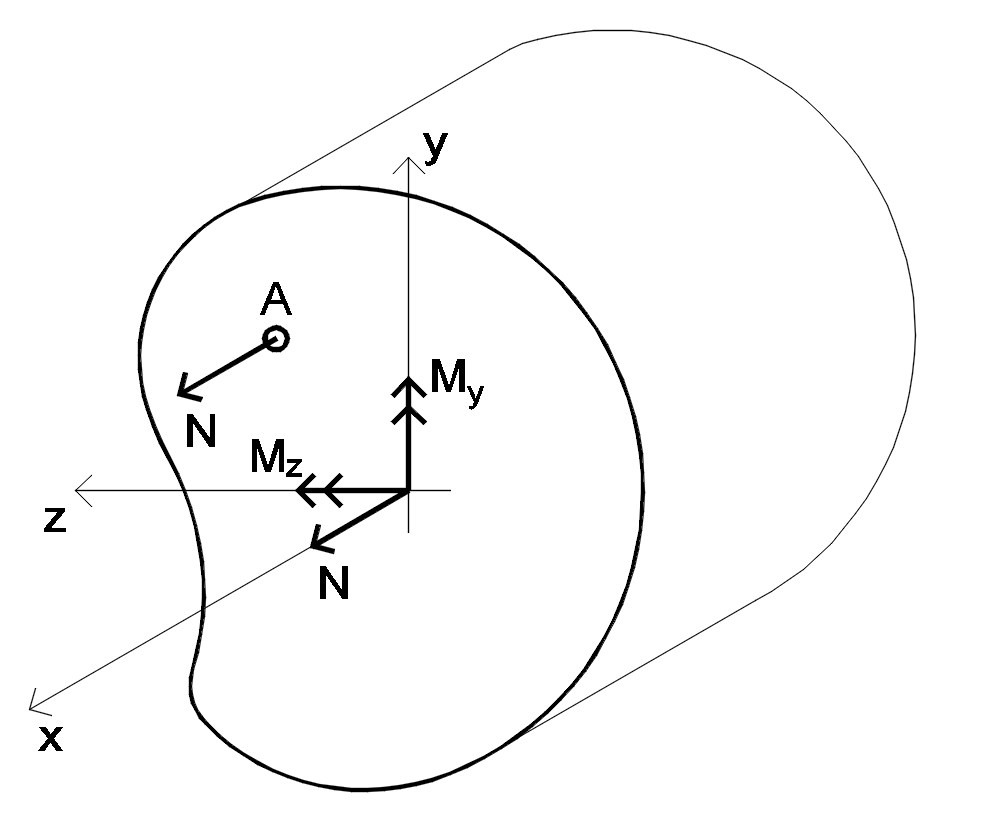
\includegraphics[width=1\textwidth]{NCesquema1HF}
\end{minipage}
\begin{minipage}{0.7\textwidth}
Expresión de tensión axial (ver ejes):
	$$
	\sigma(x,y,z)=\frac{N(x)}{A} \left (1+\frac{y_A}{\rho_z^2}y +\frac{z_A}{\rho_y^2}z\right),
\quad
	\rho_y^2=\frac{I_y}{A} ;
	\quad
	\rho_z^2=\frac{I_z}{A}.
	$$
Ecuación de la línea neutra a partir de pto. de aplicación A:
$$
1 +\frac{y_A}{\rho_z^2}y +\frac{z_A}{\rho_y^2}z=0
$$
\end{minipage}

\begin{center}
	\fcolorbox{black}{lightgray}{\textbf{Análisis seccional sin resistencia a tracción}}
\end{center}

\begin{minipage}{0.32\textwidth}
	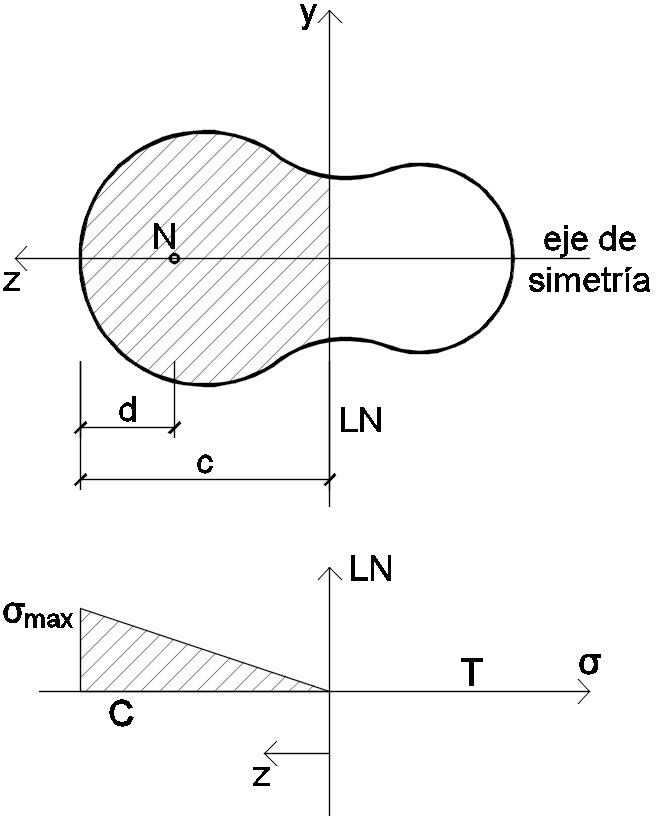
\includegraphics[width=\textwidth]{MNSTesquema1}
\end{minipage}
\begin{minipage}{0.65\textwidth}
	\hspace{0.4cm}
	Equilibrio de fuerzas y tensión en la sección:
	$$
	N=\int_{A} \sigma dA ;
	\qquad
	\sigma= k.z= -\frac{\sigma_{maxc}}{c} z
	$$
	\hspace{0.4cm}
	Equilibrio de momentos en la sección:
	$$
	N (c-d)=\int_{A} \sigma z dA ;
	$$
\end{minipage}

\vspace{0.2cm}
Caso Sección Rectangular

\begin{minipage}{0.33\textwidth}
	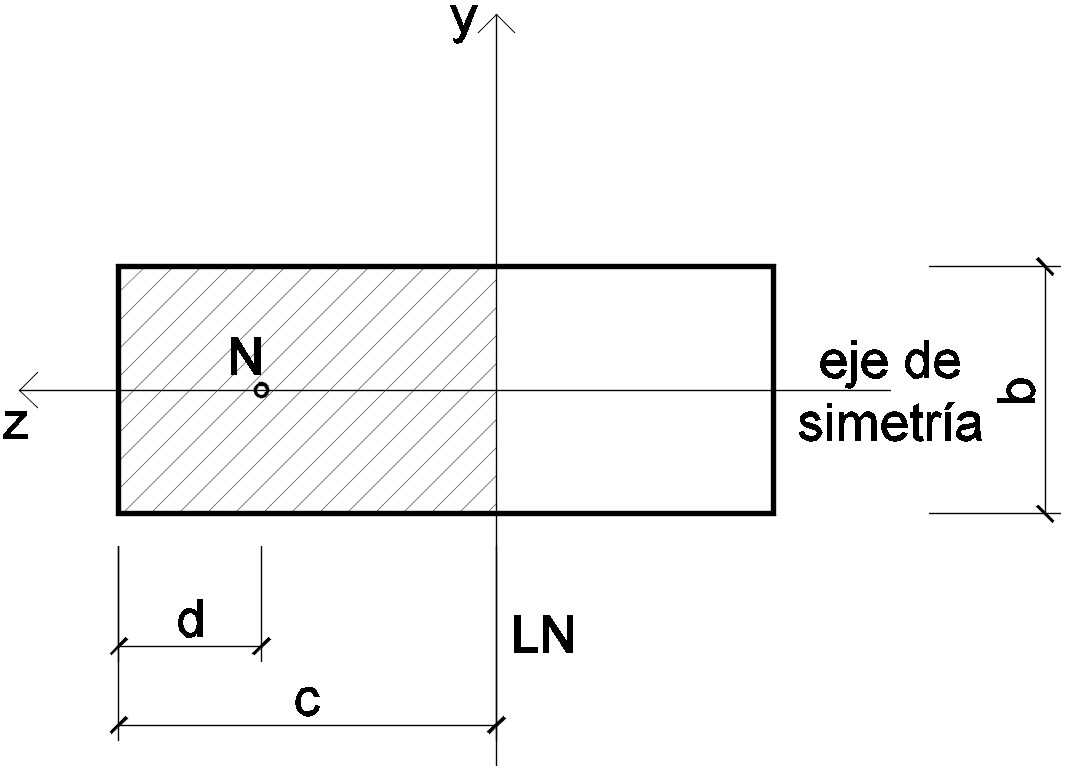
\includegraphics[width=1.3\textwidth]{MNSTrect}
\end{minipage}
\begin{minipage}{0.66\textwidth}
	\vspace{0.4cm}
	$$
	c=3d
	$$
	\vspace{0.02cm}
	$$
	N=-\frac{\sigma_{maxc}}{c}\frac{b\, c^2}{2}
	$$
	\vspace{0.02cm}
	$$
	\sigma_{maxc}=-\frac{2N}{bc}
	$$
\end{minipage}

\vspace{0.2cm}
\begin{center}
	\fcolorbox{black}{lightgray}{\textbf{Estabilidad Estructural}}
\end{center}

$$
\frac{d^2}{dx^2}\left(EI\frac{d^2 v}{dx^2}\right) + N\frac{d^2 v}{dx^2} + q =0 ;
\qquad
k^2=\frac{N}{EI}
$$

$$
\text{Caso de compresión}: v(x)= Acos(kx) + Bsin(kx) + Cx + D
$$

$$
V(x) = \frac{d}{dx}\left(EI\frac{d^2 v}{dx^2}\right) + N\frac{dv}{dx}
\qquad
M(x) = E \, I\frac{d^2 v}{dx^2}
$$


$$
\sigma_{cr,i}=\frac{E\,I\,\pi^2}{A\, {L_{p,i}}^2} ;
\qquad
L_{p,i}=\beta_i L ;
\qquad
i \, \in \, \{y,z\}
$$

$$
\sigma_{cr,i}= \frac {\pi^2 E}{{\lambda_i}^2} ;
\qquad
\lambda_i=\frac{L_{p,i}}{\rho_i} ;
\qquad
\rho_i=\sqrt{\frac{I_i}{A}}
$$

$$
\frac{M}{W} + \frac{N}{A} \leq min \{\sigma_{fluencia}, \sigma_{cr}\}
$$


\begin{center}
	\fcolorbox{black}{lightgray}{\textbf{Tabla de propiedades geométricas}}
\end{center}

\centering
\scalebox{0.62}[0.62]{
	\begin{tabular}{| c |c | c| c | c|}
		\hline
		\begin{tabular}{l}
		\end{tabular} &
		\begin{tabular}{l}
			\scalebox{2}[2]{ $I_x$} 
		\end{tabular} &
		\begin{tabular}{l}
			\scalebox{2}[2]{  $W_x$}
		\end{tabular} &
		\begin{tabular}{l}
			\scalebox{1.5}[1.5]{  $I_y$}
		\end{tabular} &
		\begin{tabular}{l}
			\scalebox{1.5}[1.5]{  $W_y$}
		\end{tabular} \\
		\hline
		\begin{tabular}{l}
			\input{./figs/HojaFormulas/rectangulo.pdf_tex}
		\end{tabular} &
		\begin{tabular}{l}
			\scalebox{2.5}[2.5]{  $\frac{bh^3}{12}$}
		\end{tabular} &
		\begin{tabular}{l}
			\scalebox{2.5}[2.5]{  $\frac{bh^2}{6}$}
		\end{tabular} &
		\begin{tabular}{l}
			\scalebox{2.5}[2.5]{  $\frac{hb^3}{12}$}
		\end{tabular} &
		\begin{tabular}{l}
			\scalebox{2.5}[2.5]{  $\frac{hb^2}{6}$}
		\end{tabular} \\
		\hline
		\begin{tabular}{l}
			\input{./figs/HojaFormulas/triangulo.pdf_tex}
		\end{tabular} &
		\begin{tabular}{l}
			\scalebox{2.5}[2.5]{  $\frac{bh^3}{36}$}
		\end{tabular} &
		\begin{tabular}{l}
			\scalebox{2.5}[2.5]{  -}
		\end{tabular} &
		\begin{tabular}{l}
			\scalebox{2.5}[2.5]{  $\frac{hb^3}{48}$}
		\end{tabular} &
		\begin{tabular}{l}
			\scalebox{2.5}[2.5]{  -}
		\end{tabular} 
		\\
		\hline
		\begin{tabular}{c}
			\input{./figs/HojaFormulas/circulo.pdf_tex}
		\end{tabular} &
		\begin{tabular}{l}
			\scalebox{2.5}[2.5]{  $\frac{\pi R^4}{4}$}
		\end{tabular} &
		\begin{tabular}{l}
			\scalebox{2.5}[2.5]{  $\frac{\pi R^3}{4}$}
		\end{tabular} &
		\begin{tabular}{l}
			\scalebox{2.5}[2.5]{  $\frac{\pi R^4}{4}$}
		\end{tabular} &
		\begin{tabular}{l}
			\scalebox{2.5}[2.5]{  $\frac{\pi R^3}{4}$}
		\end{tabular} \\
		\hline
\end{tabular}}







\newpage
\begin{table}[H]
    \centering
    \resizebox{0.95\textwidth}{!}
    {
    \begin{tabular}{m{4cm}cccc}
         \multicolumn{5}{c}{\Large Momentos de empotramiento perfecto I=cte} \\ \toprule
         %
         & \multicolumn{2}{c}{\large Empotramiento en un apoyo} & \multicolumn{2}{c}{\large Empotramiento en ambos apoyos} \\ \cmidrule{2-5} 
         %
         &  \input{./figs/TablaEmp/Mizq.pdf_tex} & \input{./figs/TablaEmp/Mder.pdf_tex} & \multicolumn{2}{c}{\input{./figs/TablaEmp/Memp.pdf_tex}} \\ \cmidrule{1-5}
        %	
        \multicolumn{1}{c}{\large{Cargas}} & \large{M} & \large{M'} & \large{M} & \large{M'} \\ \midrule
        %
        \input{./figs/TablaEmp/Caso1.pdf_tex} & $\dfrac{Qab}{2l^2}(l+b)$ &  $\dfrac{Qab}{2l^2}(l+a)$ & $\dfrac{Qab}{l^2}b$ & $\dfrac{Qab}{l^2}a$ \\ \midrule
        %
        \input{./figs/TablaEmp/Caso2.pdf_tex} & $\dfrac{3}{16}Ql$ & $\dfrac{3}{16}Ql$ & $\dfrac{1}{8}Ql$ & $\dfrac{1}{8}Ql$ \\ \midrule
        %
        \input{./figs/TablaEmp/Caso3.pdf_tex} & $\dfrac{3}{2}Qa\left(1-\dfrac{a}{l}\right)$ & $\dfrac{3}{2}Qa\left(1-\dfrac{a}{l}\right)$ & $Qa\left(1-\dfrac{a}{l}\right)$ & $Qa\left(1-\dfrac{a}{l}\right)$ \\ \midrule
        %
        \input{./figs/TablaEmp/Caso4.pdf_tex} & $\dfrac{1}{3}Ql$ & $\dfrac{1}{3}Ql$ & $\dfrac{2}{9}Ql$ & $\dfrac{2}{9}Ql$ \\ \midrule
        %
        \input{./figs/TablaEmp/Caso5.pdf_tex} & $\dfrac{15}{32}Ql$ & $\dfrac{15}{32}Ql$ & $\dfrac{5}{16}Ql$ & $\dfrac{5}{16}Ql$ \\ \midrule
        %
        \input{./figs/TablaEmp/Caso6.pdf_tex} & $\dfrac{1}{8}ql^2$ & $\dfrac{1}{8}ql^2$ & $\dfrac{1}{12}ql^2$ & $\dfrac{1}{12}ql^2$ \\ \midrule
        %
        \input{./figs/TablaEmp/Caso7.pdf_tex} & $\dfrac{qa^2}{8}\left(2-\dfrac{a}{l}\right)^2$ & $\dfrac{qa^2}{8}\left(2-\dfrac{a^2}{l^2}\right)$ & $\dfrac{qa^2}{12}\left(6-8\dfrac{a}{l}+3\dfrac{a^2}{l^2}\right)$ & $\dfrac{qa^2}{12}\left(4\dfrac{a}{l}-3\dfrac{a^2}{l^2}\right)$ \\ \midrule
        %
        \input{./figs/TablaEmp/Caso8.pdf_tex} & $\dfrac{9}{128}ql^2$ & $\dfrac{7}{128}ql^2$ & $\dfrac{11}{192}ql^2$ & $\dfrac{5}{192}ql^2$ \\ \midrule
        %
        \input{./figs/TablaEmp/Caso9.pdf_tex} & $\dfrac{qa^2}{4}\left(3-2\dfrac{a}{l}\right)$ & $\dfrac{qa^2}{4}\left(3-2\dfrac{a}{l}\right)$ & $\dfrac{qa^2}{6}\left(3-2\dfrac{a}{l}\right)$ & $\dfrac{qa^2}{6}\left(3-2\dfrac{a}{l}\right)$ \\ \midrule
        %
        \input{./figs/TablaEmp/Caso10.pdf_tex} & $\dfrac{qabc}{2l^2}\left(l+b-\dfrac{c^2}{4a}\right)$ & $\dfrac{qabc}{2l^2}\left(l+a-\dfrac{c^2}{4b}\right)$ & $\dfrac{qc}{l^2}\left[ab^2+\dfrac{c^2}{12}\left(l-3b\right)\right]$ & $\dfrac{qc}{l^2}\left[a^2b+\dfrac{c^2}{12}\left(l-3a\right)\right]$ \\ \midrule
        %
        \input{./figs/TablaEmp/Caso11.pdf_tex} & $\dfrac{qla}{16}\left(3-\dfrac{a^2}{l^2}\right)$ & $\dfrac{qla}{16}\left(3-\dfrac{a^2}{l^2}\right)$ & $\dfrac{qla}{24}\left(3-\dfrac{a^2}{l^2}\right)$ & $\dfrac{qla}{24}\left(3-\dfrac{a^2}{l^2}\right)$ \\ \midrule
        %
        \input{./figs/TablaEmp/Caso12.pdf_tex} & $\dfrac{qa^2}{120}\left(40-45\dfrac{a}{l}+12\dfrac{a^2}{l^2}\right)$ & $\dfrac{qa^2}{60}\left(10-6\dfrac{a^2}{l^2}\right)$ & $\dfrac{qa^2}{30}\left(10-15\dfrac{a}{l}+6\dfrac{a^2}{l^2}\right)$ & $\dfrac{qa^2}{20}\left(5\dfrac{a}{l}-4\dfrac{a^2}{l^2}\right)$ \\ \midrule
        %
        \input{./figs/TablaEmp/Caso13.pdf_tex} & $\dfrac{7}{120}ql^2$ & $\dfrac{1}{15}ql^2$ & $\dfrac{1}{30}ql^2$ & $\dfrac{1}{20}ql^2$ \\ \midrule
        %
    \end{tabular}
	} % end resizebox
    %\caption{Caption}
    \label{tab:empotPerf}
\end{table}


\newpage
\begin{table}[H]
	\centering
	\resizebox{0.9\textwidth}{!}
	{
		\begin{tabular}{m{4cm}cc}
			\def\svgscale{0.25}\multicolumn{3}{c}{\Large Secciones Macizas} \\ \toprule
			%
			\multicolumn{1}{c}{\large Sección} & \multicolumn{1}{c}{\large J} & \multicolumn{1}{c}{\large $W_t$} \\ \cmidrule{1-3} 
			%
			\def\svgscale{0.45}\input{./figs/TablaTorsion/fig1.pdf_tex} & $\dfrac{\pi D^4}{32}\left(1-\dfrac{d^4}{D^4}\right)$ & $\dfrac{\pi D^3}{16}\left(1-\dfrac{d^4}{D^4}\right)$ \\ \cmidrule{1-3}
			\def\svgscale{0.45}\input{./figs/TablaTorsion/fig2.pdf_tex} & $\dfrac{\pi a^3b^3}{(a^2+b^2)}$ &  $\dfrac{\pi ab^2}{2}$ \\ \cmidrule{1-3}
			\def\svgscale{0.45}\input{./figs/TablaTorsion/fig3.pdf_tex} & $\dfrac{\sqrt{3}}{80}a^4$ & $\dfrac{a^3}{20}$ \\ \cmidrule{1-3}
			\def\svgscale{0.45}\input{./figs/TablaTorsion/fig4.pdf_tex} & $\beta ab^3$ & $\alpha ab^2$ \\ \cmidrule{1-3}
			\def\svgscale{0.45}\input{./figs/TablaTorsion/fig5.pdf_tex} & $\dfrac{st^3}{3}$ & $\dfrac{st^2}{3}$ \\ \cmidrule{1-3}
			\def\svgscale{0.45}\input{./figs/TablaTorsion/fig6.pdf_tex} & $\sum_{i}^{n}\dfrac{s_it_i^3}{3}$ & $\dfrac{J}{t_{m\acute{a}x}}$ \\ \cmidrule{1-3}
			\def\svgscale{0.45}\input{./figs/TablaTorsion/fig7.pdf_tex} & $\dfrac{4\Omega^2}{\int_{s}\dfrac{ds}{t}}$ & $2\Omega t_{min}$ \\ \cmidrule{1-3}
		\end{tabular}
	} % end resizebox
	%\caption{Caption}
	\label{tab:my_label}
\end{table}

\begin{table}[H]
	\centering
	\begin{tabular}{cccccc}
		a/b & 1.00 & 1.50 & 1.75 & 2.00 & 2.50 \\ \toprule
		$\alpha$ & 0.208 & 0.231 & 0.239 & 0.246 & 0.258 \\ \cmidrule{1-6}
		$\beta$ & 0.141 & 0.196 & 0.214 & 0.229 & 0.249 \\ \cmidrule{1-6}
		$\eta$ & 1.000 & 0.859 & 0.820 & 0.795 & 0.766 \\ \cmidrule{1-6}  
	\end{tabular}
	%\caption{Caption}
	\label{tab:my_label}
\end{table}			

\begin{table}[H]
	\centering
	\begin{tabular}{ccccccc}
		a/b & 3 & 4 & 6 & 8 & 10 & $\infty$ \\ \toprule
		$\alpha$ & 0.267 & 0.282 & 0.299 & 0.307 & 0.313 & 0.333 \\ \cmidrule{1-7}
		$\beta$ & 0.263 & 0.281 & 0.299 & 0.307 & 0.313 & 0.333 \\ \cmidrule{1-7}
		$\eta$ & 0.753 & 0.745 & 0.743 & 0.742 & 0.742 & 0.742 \\ \cmidrule{1-7}  
	\end{tabular}
	%\caption{Caption}
	\label{tab:my_label}
\end{table}

